%%%%%%%%%%%%%%%%%%%%%%% file template.tex %%%%%%%%%%%%%%%%%%%%%%%%%
%
% This is a template file for The European Physical Journal
%
% Copy it to a new file with a new name and use it as the basis
% for your article
%
%%%%%%%%%%%%%%%%%%%%%%%% Springer-Verlag %%%%%%%%%%%%%%%%%%%%%%%%%%
%
\begin{filecontents}{leer.eps}
%!PS-Adobe-2.0 EPSF-2.0
%%CreationDate: Mon Jul 13 16:51:17 1992
%%DocumentFonts: (atend)
%%Pages: 0 1
%%BoundingBox: 72 31 601 342
%%EndComments

gsave
72 31 moveto
72 342 lineto
601 342 lineto
601 31 lineto
72 31 lineto
showpage
grestore
%%Trailer
%%DocumentFonts: Helvetica
\end{filecontents}
%
\documentclass[epj]{svjour}
%\documentclass[epj, referee]{svjour}
% Remove option referee for final version
%
% Remove any % below to load the required packages
%\usepackage{latexsym}
\usepackage{enumitem}
\usepackage{float}
\usepackage{amsmath}
% \usepackage[sorting=none]{biblatex}
% \bibliography{biblio}
\usepackage{graphics}
\usepackage{graphicx}
% etc
%
% \setlength\parskip{\baselineskip}
\begin{document}
%
\title{Lightweight pulse-shape analysis method using a machine learning ensemble algorithm on an AGATA detector}
% \subtitle{Do you have a subtitle?\\ If so, write it here}
\author{Antoine Corbel\inst{1}, Damian Ralet\inst{2}, Mohamad Moukaddam\inst{1}, Gilbert Duchêne\inst{1}, Michaël Ginsz\inst{2}} % etc
% \thanks is optional - remove next line if not needed
% \thanks{\emph{Present address:} Insert the address here if needed}%
%}                     % Do not remove
%
% \offprints{}          % Insert a name or remove this line
%
\institute{Université de Strasbourg, CNRS, IPHC UMR 7178, F-67000 Strasbourg, France \and Mirion Technologies CANBERRA (SAS), Lingolsheim, France}
%
\date{Received: date / Revised version: date}
% The correct dates will be entered by Springer
%
\abstract{
Pulse-shape analysis (PSA) techniques are widely used with segmented HPGe detectors for $\gamma$-ray tracking purposes, such as in the AGATA (Advanced GAmma Tracking Array) collaboration. It utilizes a simulated basis of pulses taking advantage of the position sensitivity of segmented HPGe detectors to determine the interaction position, which is needed for $\gamma$-ray tracking and Doppler correction. The typical approach of PSA is computationally expensive and thus incompatible with embedded electronics such as a moderate-spec laptop. This work presents an algorithm using an ensemble machine learning model, gradient boosted regression trees, to reconstruct the 3D position of an interaction based on features extracted from its pulse, such as rise time and transient signal integrals. Construction and training of the models is presented as well as performance evaluation on a collimated beam of $^{137}$Cs at 662 keV, events being reconstructed both at fold-1 and 2 (single and double-hit events, respectively), in a 36-fold segmented AGATA detector.
%
\PACS{
      {AGATA spectrometer:} {gamma-ray tracking array for nuclear physics};
      {HPGe detectors:} {segmented detectors used in AGATA};
      {Pulse Shape Analysis:} {refining interactions position in the detector};
      {Gradient boosted trees:} {combining regression trees to predict interaction positions};
     } % end of PACS codes
} %end of abstract
%
\authorrunning{Corbel A.}
\titlerunning{Ligthweight PSA machine learning model}
\maketitle
%
\section{Introduction}
\label{sec:intro}
In state-of-the-art HPGe segmented detectors, such as in international collaborations Advanced GAmma Tracking Array (AGATA)~\cite{Akkoyun2012} and Gamma-Ray Energy Tracking Array (GRETA)~\cite{Lee2003DevelopmentsArrays}, the interaction position of the $\gamma$-ray can be determined from the signal pulse in the hit segment and transient pulses in the neighbouring segments (see \textbf{Fig.}~\ref{fig:a005_geometry} for segmentation pattern). The $\gamma$-ray interaction positions and energy deposits are used by tracking algorithms~\cite{Bazzacco:2004nnw,Lopez-Martens2004}  to determine the Compton sequencing of the photon inside the detector. The approach followed by the AGATA collaboration was so far to simulate, using the AGATA Data Library (ADL)~\cite{Bruyneel2006,Bruyneel2006-2,BruyneelUnpub}, a basis of pulses associated to positions on a 2~mm Cartesian grid in the 3D volume of the germanium detector. The experimentally measured signal is then compared to the basis to determine the interaction position.

The present work uses a 3D scanned basis built with data from the IPHC scanning table and the Pulse-Shape Comparison Scan (PSCS) method~\cite{Crespi2008}. Instead of comparing the super-pulses~\cite{}, the approach presented in this paper uses a subset of features extracted from the pulses to locate the $\gamma$-ray interaction. Multiple gradient boosting models are trained on the features of the scanned 3D basis and takes as inputs features from measured pulses, to predict the interaction position.

After introducing the dataset in \textbf{Section} \ref{sec:dataset_building}, the model and its training is presented in \textbf{Section }\ref{sec:models_training}. Model evaluation is performed in \textbf{Section} \ref{sec:results} and position reconstruction results, evaluated using pulses of an unseen dataset, from interactions of a collimated beam of 662 keV $\gamma$-rays in an AGATA crystal, are shown in \textbf{Section} \ref{sec:position_reconstruction}.

\section{Dataset building}
\label{sec:dataset_building}
The dataset used in this work was generated from the IPHC scanning table, that uses the Pulse Shape Comparison Scanning (PSCS) method~\cite{Crespi2008}. To build the dataset of pulses in the volume of the AGATA detector A005 (shown in \textbf{Fig.}~\ref{fig:a005_geometry}), a collimated beam of 662 keV $\gamma$ rays from a $^{137}$Cs source was moved by a step of 2~mm along both scanning table axes. The vertical scan is composed of 1305 scanned positions in the XY-plane of the detector's coordinate system (denoted as (\textbf{X}\textsubscript{c},\textbf{Y}\textsubscript{c},\textbf{Z}\textsubscript{c}) in figures and text). The horizontal scan is composed of 1866 scanned positions in the XZ-plane of the detector. IPHC scanning table is equipped with 10 TNT2-D, 14 bits-100 MHz, digital electronic cards~\cite{Arnold2005} for data acquisition. For each interaction, $120$ samples are saved, around the leading edge of the 37 pulses (36 segments and 1 total energy signal).

\begin{figure}
\centering
\resizebox{0.45\textwidth}{!}{%
  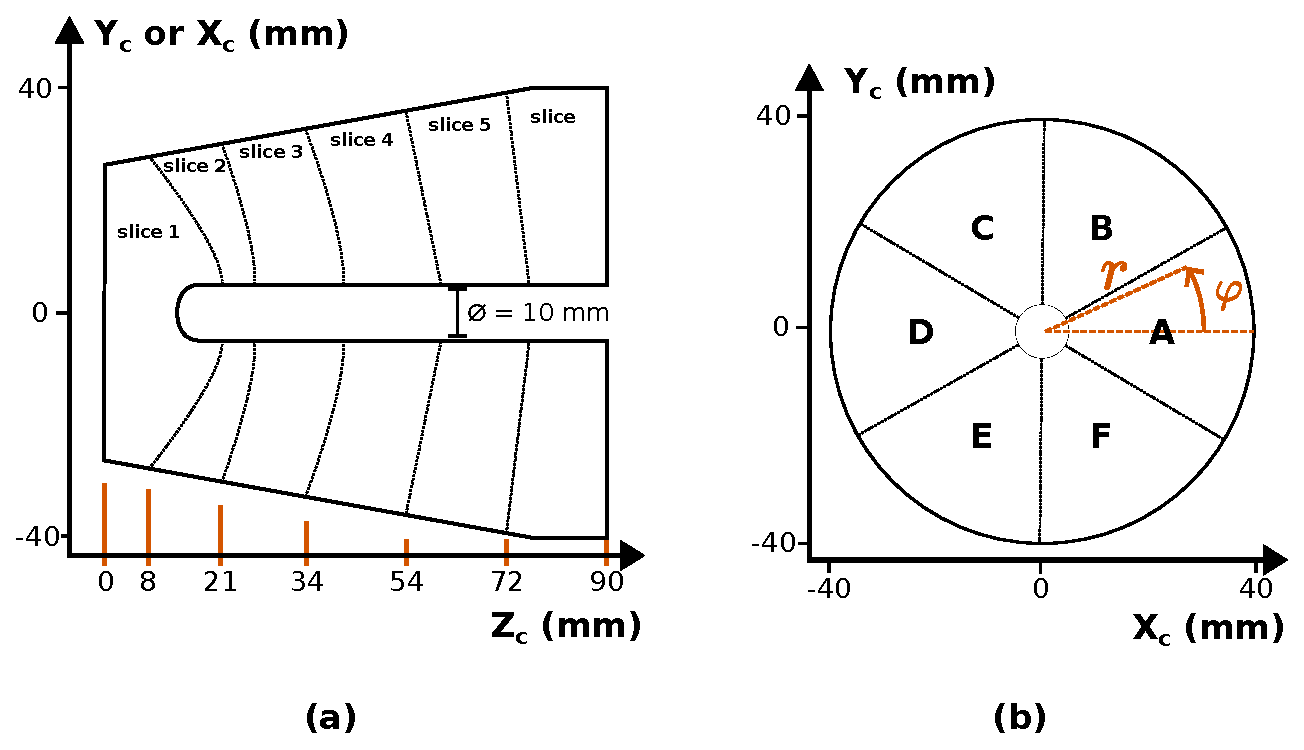
\includegraphics{images/A005_geom_with_lengths_Rhole10_newGeom.eps}
}
\caption{\textbf{(a)} Longitudinal section of A005. Slices are labelled from 1 (front of the detector) to 6 (back). \textbf{(b)} Transverse section of A005. Sectors are labelled from A to F (view from the back). Each slice has 6 sectors, for a total of 36 segments. Cylindrical coordinates $r, \varphi, \text{Z}_\text{c}$ are represented. }
\label{fig:a005_geometry}
\end{figure}

Both scans were calibrated and gain matched to ensure pulses of both scans could be compared with $\chi^2$ minimisation method, see~\cite{DeCanditiis2020SimulationsDetector} for details. A gate of 3 keV around the 661.7 keV photoelectric peak of $^{137}$Cs was applied to compare full-energy deposition pulses. Due to the position sensitivity of HPGe detectors, pulses will differ between vertical and horizontal scans except at crossing points. Crossing both scan grids allows to reconstruct a pulse for all 36 segments of the detector and the core contact, at 47 000 positions. 

The pitch of both scans being 2~mm results in an equally 2~mm spaced points in the 3D basis, along all cartesian axes.

% In this work, all 36 segments are referenced by a segment ID. \textbf{Table}~\ref{tab:segment_mapping} maps segment ID to the conventional AGATA notation using sector labels from A to F and slice numbers from 1 to 6. Note that the core is assigned to ID = 0.

% % MAPPING AGATA TO SEG ID TABLE
% \begin{table}[h]
% \centering
% \caption{Mapping of AGATA segment convention to the one used in this work. ID = 0 is reserved to the core contact.}
% \label{tab:segment_mapping}       % Give a unique label
% \begin{tabular}{lcccccc}
% \hline\noalign{\smallskip}
% \textbf{Slice} & \textbf{A} & \textbf{B} & \textbf{C} & \textbf{D} & \textbf{E} & \textbf{F} \\
% \noalign{\smallskip}\hline\noalign{\smallskip}
% 1 (tip) & 1  & 7  & 13 & 19 & 25 & 31 \\
% 2       & 2  & 8  & 14 & 20 & 26 & 32 \\
% 3       & 3  & 9  & 15 & 21 & 27 & 33\\
% 4       & 4  & 10 & 16 & 22 & 28 & 34 \\
% 5       & 5  & 11 & 17 & 23 & 29 & 35 \\
% 6 (back) & 6 & 12 & 18 & 24 & 30 & 36 \\
% \noalign{\smallskip}\hline
% \end{tabular}
% \end{table}

\begin{figure}
\centering
\resizebox{0.48\textwidth}{!}{%
  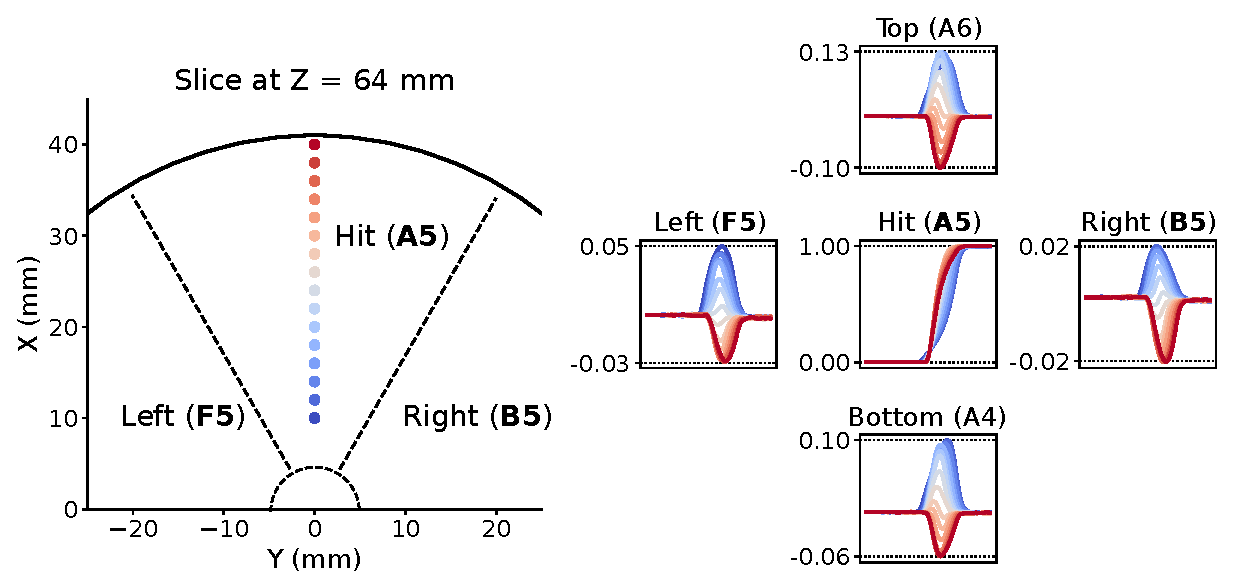
\includegraphics{images/seg5_Z64mm_Ycst_rotated_Rhole10.eps}
}
\caption{Normalized pulse shapes from points in the XY-plane of A005 detector, along X-axis, in segment A5. The color gradient shows the position dependence of the pulses shapes in the detector. Transient signals are also drawn to emphasize their radial dependence. Top and bottom neighbor signals are from segments A6 and A4. Left and right transient signals are from segments F5 and B5, respectively.}
\label{fig:neighbors_Ycst}
\end{figure}

\subsection{Features extraction}
\label{subsec:feature_extraction}

Instead of utilizing a performant but computationally intensive grid-search algorithm (or the adaptative grid-search algorithm) as used in AGATA~\cite{Venturelli2004}, relevant features are extracted from the pulses of the hit segment, its four closest neighbors (top, down, left and right) and the core, providing the model enough information on the position of the interaction in the detector volume. The aim is to use a lighter PSA method, to allow usage of the model on an embedded software. Given the quasi-rotational symmetry of A005 (the crystal is asymmetric), a cylindrical coordinate system $(r, \varphi, z)$ is adopted.

The first feature that is used is the segment ID of the hit segment (named \textit{SegID}). A005 having 36 segments, this information alone refines the position to a few cm$^3$. To bring additional depth information, the slice number (named \textit{SliceID}) illustrated in \textbf{Fig.}~\ref{fig:a005_geometry}(a) is also used as a feature.

\begin{figure}
\centering
\resizebox{0.48\textwidth}{!}{%
  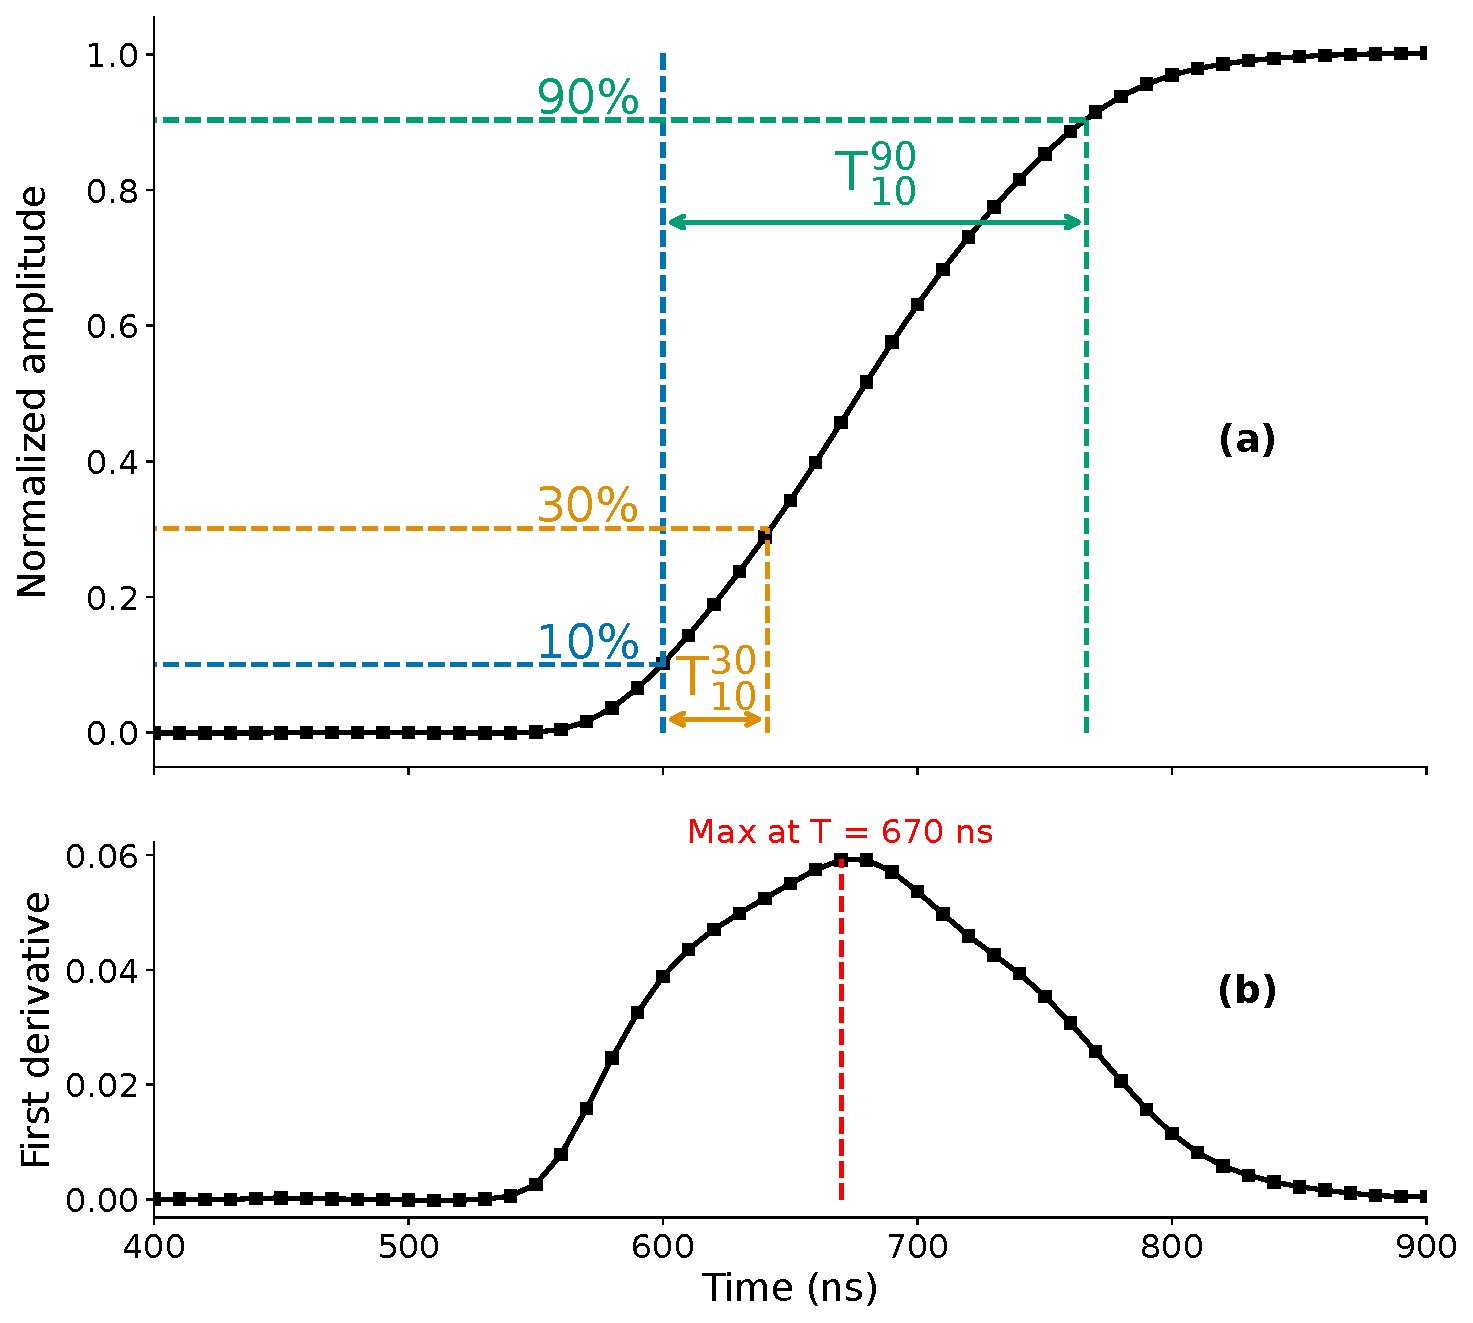
\includegraphics{images/pulse_T30_T90_deriv_subplot_cblind.eps}
}
\caption{\textbf{(a)} Illustration of both T$^{30}_{10}$ and T$^{90}_{10}$ rise times on a pulse. \textbf{(b)} First derivative of the above pulse and annotation for the time at which the maximum of the derivative is reached (red dashed vertical line).}
\label{fig:pulse_t30_t90}
\end{figure}

\subsubsection{Radial ($r$) related features}
The rise-time feature of a pulse correlates with the radius of the interaction position. It corresponds to the time taken by a pulse to go from 10\% to $x$\% (denoted as T$^{x}_{10}$) of its total amplitude, $x$ being an arbitrary amplitude value. It derives from the charge carriers drift time in the detector, directly linked to the radius of the interaction in a coaxial detector such as A005. The evolution of the pulse shape of the hit segment and its four closest neighbors is depicted in \textbf{Fig.}~\ref{fig:neighbors_Ycst}. Both T$^{30}_{10}$ and T$^{90}_{10}$ are used as features in this work (see \textbf{Fig.}~\ref{fig:pulse_t30_t90}a), as they give complementary information about the interaction radius.
The time at which the derivative of the hit-segment's pulse reaches its maximum (named \textit{MaxDerivTime}) is also correlated to the radius of the interaction, it is thus used as an input for the model (\textbf{Fig.}~\ref{fig:pulse_t30_t90}b).

\subsubsection{Azimuthal angle ($\varphi$) related features}
An azimuthal information is obtained by looking at the neighbors transient pulses. By computing the integral of the left and right transient signals (see \textbf{Fig.}~\ref{fig:neighbor_signals_RadCst}), one can refine the azimuthal position of the interaction within a segment.

\begin{figure}
\centering
\resizebox{0.48\textwidth}{!}{%
  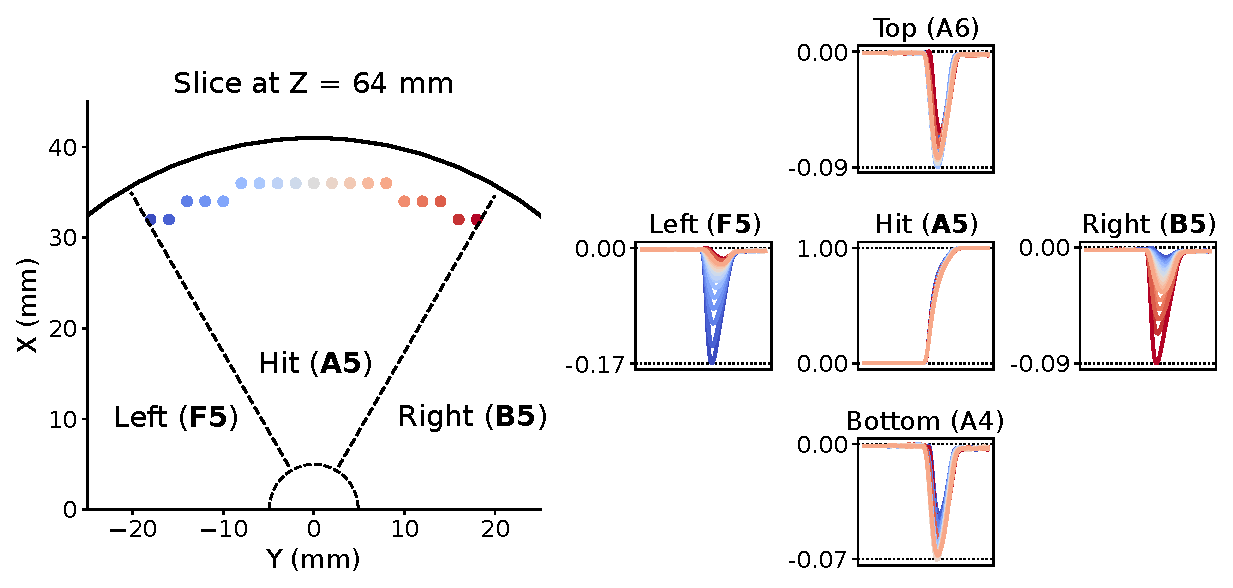
\includegraphics{images/seg5_Z64mm_RadiusCst_rotated_Rhole10.eps}
}
\caption{Normalized pulse shapes from points in the XY-plane
of A005 detector, along X-axis, in segment A5. The hit positions shown have a radius varying from $35$ mm to $37$ mm. The influence of the azimuthal angle of the hit on the neighbors transient signals is shown.}
\label{fig:neighbor_signals_RadCst}
\end{figure}

The absolute integral is the sum of the absolute values of the 120 samples of a pulse. Features computed using this method are named \textit{Up-}, \textit{Down-}, \textit{Left-} and \textit{Right-} integrals. Similarly, polarity of the transient signals can be integrated in the model by summing samples without using their absolute value. The polarity can help refine the radius of the interaction, as seen in \textbf{Fig.}~\ref{fig:neighbors_Ycst} with the polarity inversion occurring as $r$ grows. These features are called \textit{Up-}, \textit{Down-}, \textit{Left-} and \textit{Right-Polarity} in subsequent figures.

\subsubsection{Depth ($z$) related features}
The depth of the interaction within the crystal, following the $z$ coordinate, can be refined through the use of the transient signals of the bottom and top neighbours (see \textbf{Fig.}~\ref{fig:neighbors_Ycst}). Similarly, both the magnitude and the polarity are taken into account for those signals.

% \subsection{Subsection title}
% \label{sec:2}
% as required. Don't forget to give each section
% and subsection a unique label (see Sect.~\ref{sec:1}).
% %
% % For one-column wide figures use
% \begin{figure}
% % Use the relevant command for your figure-insertion program
% % to insert the figure file.
% % For example, with the option graphics use
% \resizebox{0.75\textwidth}{!}{%
%   \includegraphics{leer.eps}
% }
% % If not, use
% %\vspace{5cm}       % Give the correct figure height in cm
% \caption{Please write your figure caption here}
% \label{fig:1}       % Give a unique label
% \end{figure}

\section{Models training}
\label{sec:models_training}
The chosen model for this work is gradient boosted regression trees (GBRT)~\cite{Friedman2001GreedyMachine.}. It is an ensemble model that improves the performances of regression trees by iteratively combining them. 

\subsection{Regression trees}
Regression trees work by recursively partitioning the feature space based on feature values. Each tree split is chosen to minimize a loss function within each partition, such as the root mean squared error (RMSE) chosen in this work. For $n$ samples, RMSE is defined as 

\begin{equation}
\label{eq:rmse}
    \operatorname {RMSE} = \sqrt{\frac{1}{n}\sum _{i=1}^{n}\left(Y_{i}-{\hat {Y_{i}}}\right)^{2}},
\end{equation}

where $Y_{i}$ and $\hat {Y_{i}}$ are the expected (true) and the predicted values, respectively.


This partition splits the feature space into two distinct regions that can be further partitioned. Each partition adds depth to the regression tree, making it more complex. Parameters such as tree depth, minimum samples to split a node (M\textsubscript{S}) or minimum samples in a leaf (M\textsubscript{L}), shown in \textbf{Fig.}~\ref{fig:regression_tree}, can help reduce the complexity of a tree by limiting its ability to create too specific partitions. 

\begin{figure}
\centering
\resizebox{0.48\textwidth}{!}{%
  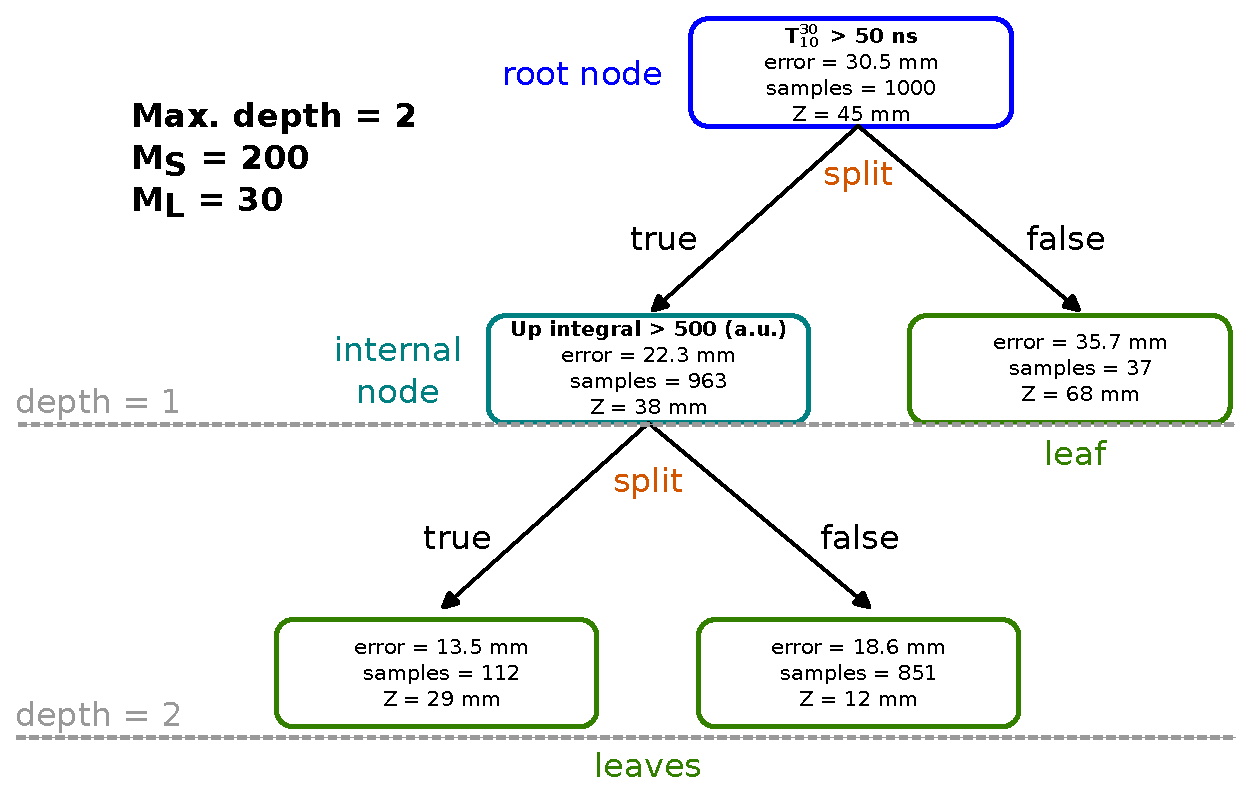
\includegraphics{images/regression_tree_depth.eps}
}
\caption{Illustration of a single regression tree, hypothetically predicting the depth ($Z$) of the interaction within the detector, for explanatory purposes only. The subset of features used is the rise time to 30\% of the maximum amplitude (T$_{10}^{30}$) and the upper-neighbor transient-signal integral using absolute value (\textit{Up-} integral). Hypothetical tree parameters depth, M\textsubscript{S} and M\textsubscript{L}, explained in the text, are also given. The error is computed using \textbf{Eq.} \ref{eq:rmse}.}
\label{fig:regression_tree}
\end{figure}

A leaf is a node of the tree that does not have sub-partitions. However, even with tuned parameters, standalone regression trees are prone to overfitting and may not generalize to unseen data.

\subsection{Gradient boosted regression trees}

GBRT adress this problem by building trees sequentially, each new tree correcting the residuals (prediction error) of the previous tree. The predictions of each tree are scaled by a learning rate which controls the contribution of each tree to the final prediction. Additional parameters, such as the random fraction of training data used to train each tree and the maximum number of features used for each tree, introduce randomness to reduce overfitting of the model.

\subsection{Targets}

The objective of this work is to predict the position of an interaction in 3D space, represented as a vector $[r, \varphi, z]$, using extracted features given as inputs to the model. Instead of training a single multi-output model to predict all coordinates simultaneously, separate models are trained for each coordinate as this has resulted in better performances (lower 3D euclidean error) in preliminary model trainings done in the course of this work.

Special attention is required for the azimuthal angle $\varphi$, as it is a cyclic angle with values in $[0, 2\pi]$. A classical loss function, such as the RMSE used in this work, would incorrectly compute high residual values to predictions near the boundaries of this range (e.g. $Y = 0$ and $\hat Y = 2\pi$).
To address this issue, $\varphi$ is encoded into two components, $\sin \varphi$ and $\cos \varphi$, which both lie in $[-1, 1]$ range, effectively avoiding the cyclic nature of the $\varphi$ angle. Even though $\sin \varphi$ and $\cos \varphi$ are not independent since they satisfy the relationship $\sin^2 \varphi + \cos^2 \varphi = 1$, the two models used to predict them are independent, meaning the relationship does not strictly hold. The azimuthal angle reconstruction has shown better results using this mapping rather than using $\varphi$ coordinate without transformation. The predicted $\varphi$ angle is then recomputed using 
\begin{equation}
\label{eq:atan2}
    \varphi = \operatorname{arctan}_2(\sin \varphi, \cos \varphi),
\end{equation}
where $\operatorname{arctan}_2$ is a modified $\arctan$ function that returns values in $[-\pi, \pi]$ instead of $[-\frac{\pi}{2}, \frac{\pi}{2}]$, covering all four quadrants of the unit circle. The result can then be adjusted to the original range $[0, 2\pi]$ of the $\varphi$ angle.

In total, four separate models are trained on of 90\% of the A005 pulses database. The 10\% left constitute the test dataset that is used to evaluate the model's performance on unseen data, after training.

\textbf{Fig.}~\ref{fig:corr_matrix} shows the Pearson correlation coefficients for all pairs of variables (features and targets). It allows to capture the linear relationship between two variables. If one of the two variables is a target of the model, the higher the coefficient the more the feature will help having a good model. If the two compared variables are features, a higher (or lower) coefficient indicates that both variables will bring similar information to the model, and using only one could be best. Pearson's correlation coefficient between two variables X and Y is computed using:

\begin{equation}
    \rho_{X,Y}={\frac {\operatorname {cov} (X,Y)}{\sigma _{X}\sigma _{Y}}},
\end{equation}

where $\operatorname{cov}$ is the covariance, $\sigma_X$ and $\sigma_Y$ are the standard deviations of the X and Y variables, respectively.
Using an ensemble model has for objective to model non-linear phenomena, as is the position-dependence of the pulses shapes. Thus, even though some features have linear correlation coefficients near 0 with targets, this does not rule out non-linear correlations.

\begin{figure}
\centering
\resizebox{0.48\textwidth}{!}{%
  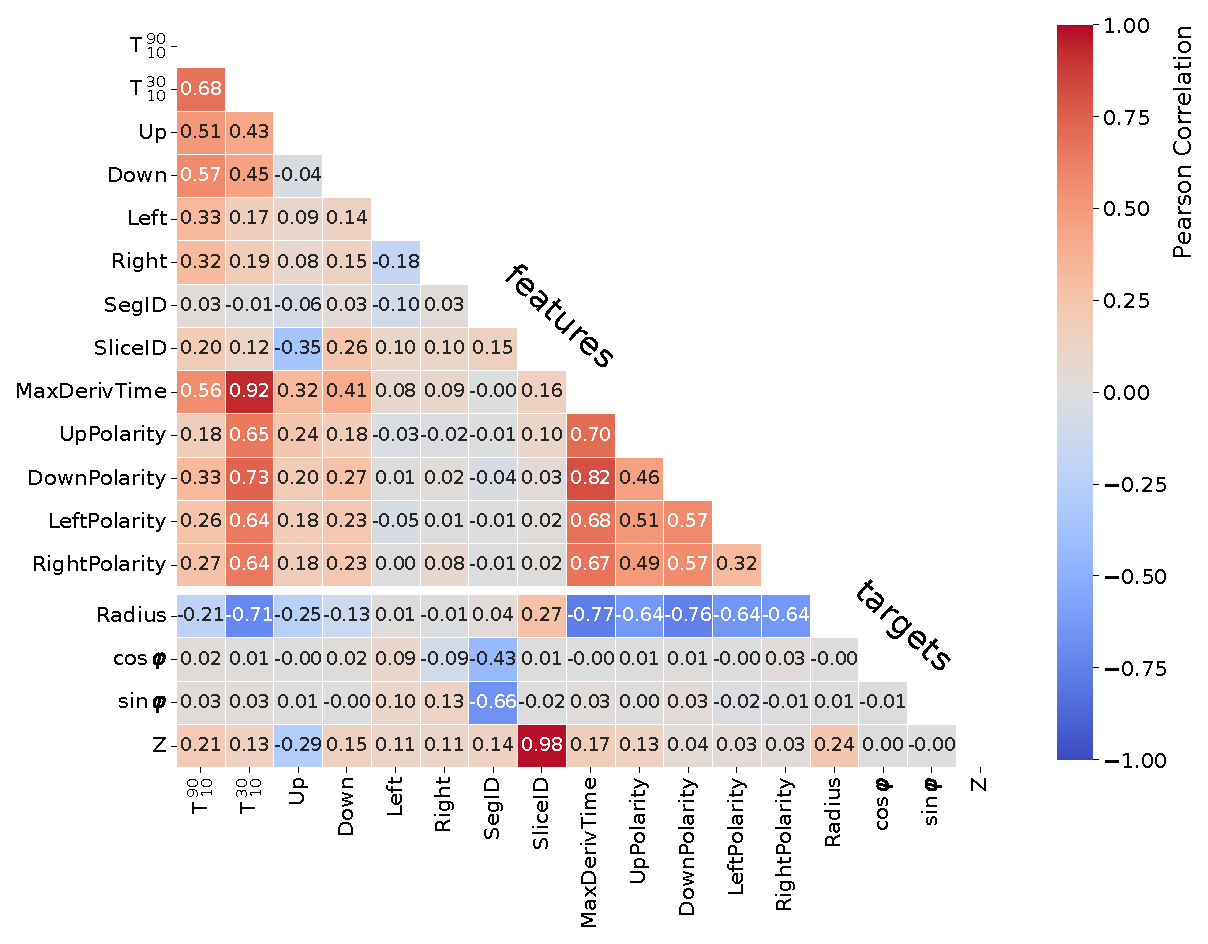
\includegraphics{images/corr_mat_mod.eps}
}
\caption{Correlation matrix of the model's features and targets. Pearson's correlation coefficient for each pair of variable is displayed. It represents the linear correlation between the two elements of each pair. Features ``\textit{Up}'', ``\textit{Down}'', ``\textit{Left}'' and ``\textit{Right}'' correspond to the absolute value integrals of the transient signals.}
\label{fig:corr_matrix}
\end{figure}

\subsection{Training curves}
Training curves are used to monitor the performance of the GBRT models during the training phase. Hyper-parameter tuning is done using bayesian optimisation~\cite{Akiba2019}, with the RMSE as the loss function on the validation set. For each constructed tree, 10\% of the samples dedicated to the training of the tree is randomly kept aside as a validation set. These are used to evaluate tree performance during the training phase of the model, also allowing to monitor overfitting by comparing the training and validation curves evolution as new trees are created (see \textbf{Fig.}~\ref{fig:all_losses_curves}). 

An early-stopping criterion is used to stop the training after 10 new trees without improvement of the loss function on the validation set, further limiting the risk of overfitting.
% % For one-column wide figures use
\begin{figure}[h]
\centering
\resizebox{0.48\textwidth}{!}{%
  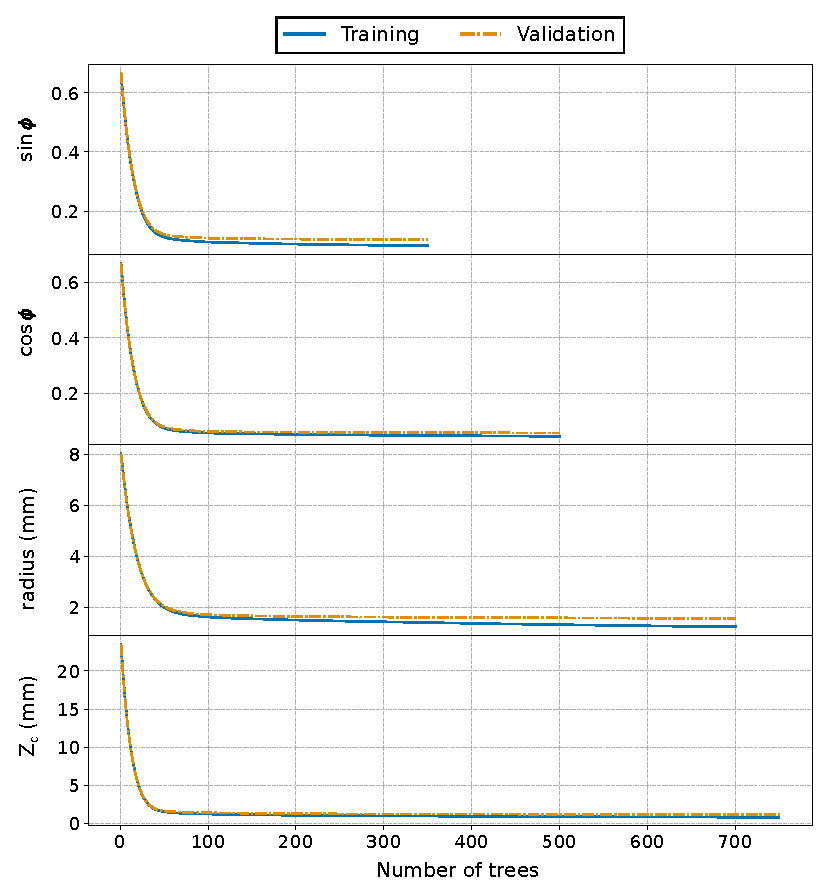
\includegraphics{images/gbdt_losses.eps}
}
% If not, use
%\vspace{5cm}       % Give the correct figure height in cm
\caption{All targets training and validation losses with increasing number of trees. The metric being minimised is  the root mean squared error (RMSE), evaluated on per-tree validation sets. Early stopping after 10 trees without improvement on the validation loss is used to prevent overfitting.}
\label{fig:all_losses_curves}       % Give a unique label
\end{figure}

% The RMSE values for the train set are gathered in \textbf{Table}~\ref{tab:train_metrics}.

% \begin{table}[h]
% \centering
% \caption{Train set metrics. Units are given  in mm for radius and Z, unitless for $\sin \varphi$ and $\cos \varphi$.}
% \label{tab:train_metrics}       % Give a unique label
% \begin{tabular}{lll}
% \hline\noalign{\smallskip}
% Target & RMSE & R$^2$  \\
% \noalign{\smallskip}\hline\noalign{\smallskip}
% Radius & 1.2418 & N/A \\
% $\sin \varphi$ & 0.0828 & N/A \\
% $\cos \varphi$ & 0.0446 & N/A \\
% Z & 0.8147 & N/A \\
% \noalign{\smallskip}\hline
% \end{tabular}
% \end{table}

% \begin{table}
% \caption{Metrics for Model Performance on Training and Test Sets}
% \label{tab:model_metrics}       % Give a unique label
% \begin{tabular}{llll}
% \hline\noalign{\smallskip}
% Target & Dataset & Metric & Value  \\
% \noalign{\smallskip}\hline\noalign{\smallskip}
% Radius & Train & RMSE & 1.2418 \\
% Radius & Test & RMSE & 1.4828 \\
% Radius & Test & R² & 0.9679 \\
% $\sin \varphi$ & Train & RMSE & 0.0828 \\
% $\sin \varphi$ & Test & RMSE & 0.0869 \\
% $\sin \varphi$ & Test & R² & 0.9846 \\
% $\cos \varphi$ & Train & RMSE & 0.0446 \\
% $\cos \varphi$ & Test & RMSE & 0.0550 \\
% $\cos \varphi$ & Test & R² & 0.9941 \\
% $\varphi$ & Test & RMSE & 6.1329 \\
% $\varphi$ & Test & MAE & 2.7381 \\
% Z & Train & RMSE & 0.8147 \\
% Z & Test & RMSE & 1.1416 \\
% Z & Test & R² & 0.9980 \\
% 3D Euclidean Distance & Test & Mean & 1.7742 \\
% 3D Euclidean Distance & Test & Median & 1.2619 \\
% \noalign{\smallskip}\hline
% \end{tabular}
% \end{table}
\subsection{Feature importance}

To understand how input features impact the target prediction, SHAP (Shapley Additive exPlanations) method is used~\cite{lundberg2017}. For a chosen subset of points from the test-set (100 in this work, enough to see patterns in the feature importance graphs), predictions are recomputed by removing one feature from the input set and observing how the prediction is affected. It gives insights on the model that was trained and the importance of each feature. \textbf{Fig.}~\ref{fig:detph_treeSHAP} presents the prediction of $z$, the depth of the interaction, for all features of the model and the impact of each feature's value on the prediction.

\begin{figure}
\centering
\resizebox{0.48\textwidth}{!}{%
  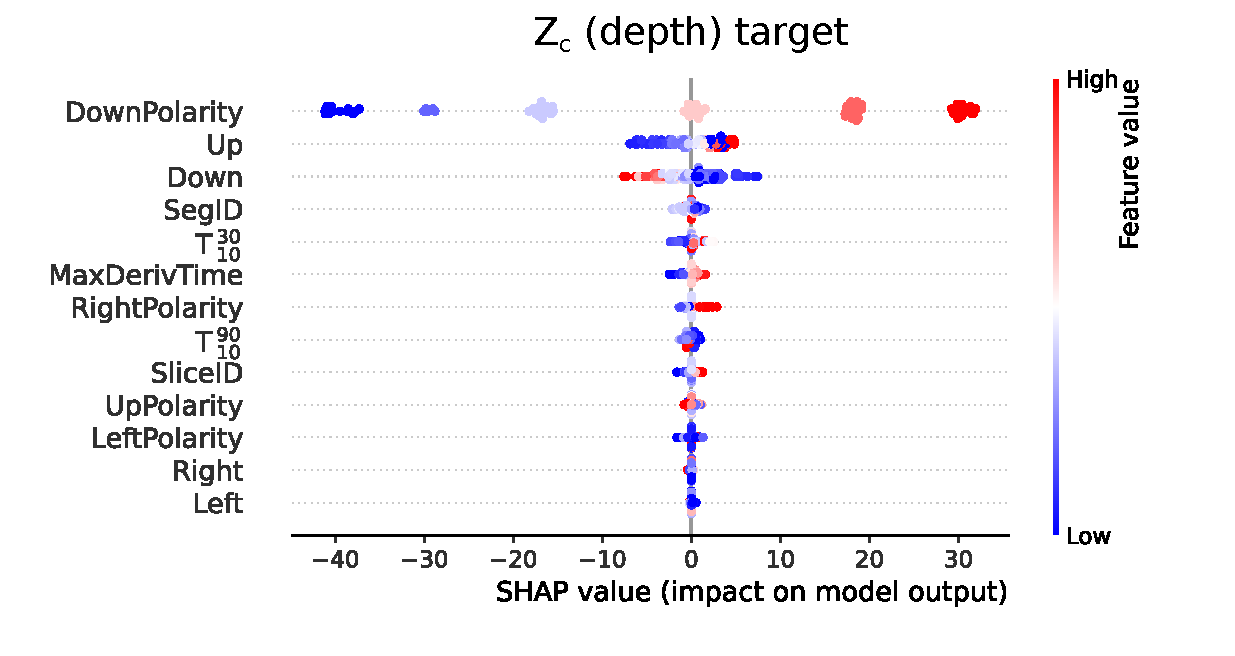
\includegraphics{images/Z_treeShap.eps}
}
% If not, use
%\vspace{5cm}       % Give the correct figure height in cm
\caption{Depth model feature importance, sorted by descending order from top to bottom. Color scale indicates the intensity of the feature value, from lowest (blue) to highest (red). X-axis 0~value is the baseline of the model. Six clusters can be observed for the \textit{DownPolarity} feature, representing the six slices of the detector.} 
\label{fig:detph_treeSHAP}       % Give a unique label
\end{figure}

The feature \textit{DownPolarity} has the most impact on the predictions of the model. Six clusters are observed, one for each slice of A005 detector. Low values of polarity are shown in blue and high values in red. The second most important feature for depth prediction is the upper segment integral (\textit{Up}). This feature importance analysis is insightful as it can be observed that the most impactful feature for depth ($z$) prediction is not the \textit{sliceID} as the correlation matrix in \textbf{Fig.}~\ref{fig:corr_matrix} indicated.

%Other models' feature importance graphs are shown in appendix (TODO).

% To understand the impact of each input feature on the predictions of the GBRT model, we employed TreeSHAP, a powerful tool designed to explain the contribution of individual features to the model’s output for each target variable (Radius, $\varphi$, and Z). TreeSHAP works by breaking down a prediction into the specific influences of each feature, showing how much each one pushes the prediction away from a baseline value—think of it as assigning a "credit" or "blame" to each feature for the final result, based on its value in a given data point. This method reveals not only which features are most important overall, as visualized in bar charts that rank features by their average impact on predictions, but also how the effect of each feature varies across different data points, as shown in beeswarm plots that display the distribution of a feature’s influence alongside its values (e.g., whether high or low values of a feature consistently increase or decrease the prediction). Mathematically, TreeSHAP calculates SHAP (SHapley Additive exPlanations) values for each feature i in a prediction, representing its marginal contribution as:

% \begin{equation}
% \label{eq:shap}
% \phi_i = \sum_{S \subseteq N \setminus {i}} \frac{|S|!(|N|-|S|-1)!}{|N|!} \left[ f(S \cup {i}) - f(S) \right],
% \end{equation}

% Using Shapley values~\cite{Lundberg2018}, it is possible to understand what features were the most important for a good prediction of the model. On a random sample of the test set, models are predicting their target variable with and without a specific feature of the set. The predictions are then compared and the impact of this specific feature can be quantified.

\section{Test-set and real-case results}
\label{sec:results}
\subsubsection*{\underline{Models residuals}}

After training the model, it is evaluated on the test-set, constituting 10\% of the total dataset that the model has not seen during the training phase. The residuals are computed as $\sum_{i=1}^n Y_i - \hat Y_i$ 
with $n$ the number of samples of the test-set. \textbf{Fig.}~\ref{fig:all_residuals} gathers $[r, \varphi,z]$ residuals after recombination of $\varphi$ from $\sin \varphi$ and $\cos \varphi$ using \textbf{eq.} \ref{eq:atan2} and conversion from radians to degrees. \textbf{Table}~\ref{tab:rmse_metrics} gives the RMSE value for both training and testing sets.
% For two-column wide figures use
\begin{figure*}
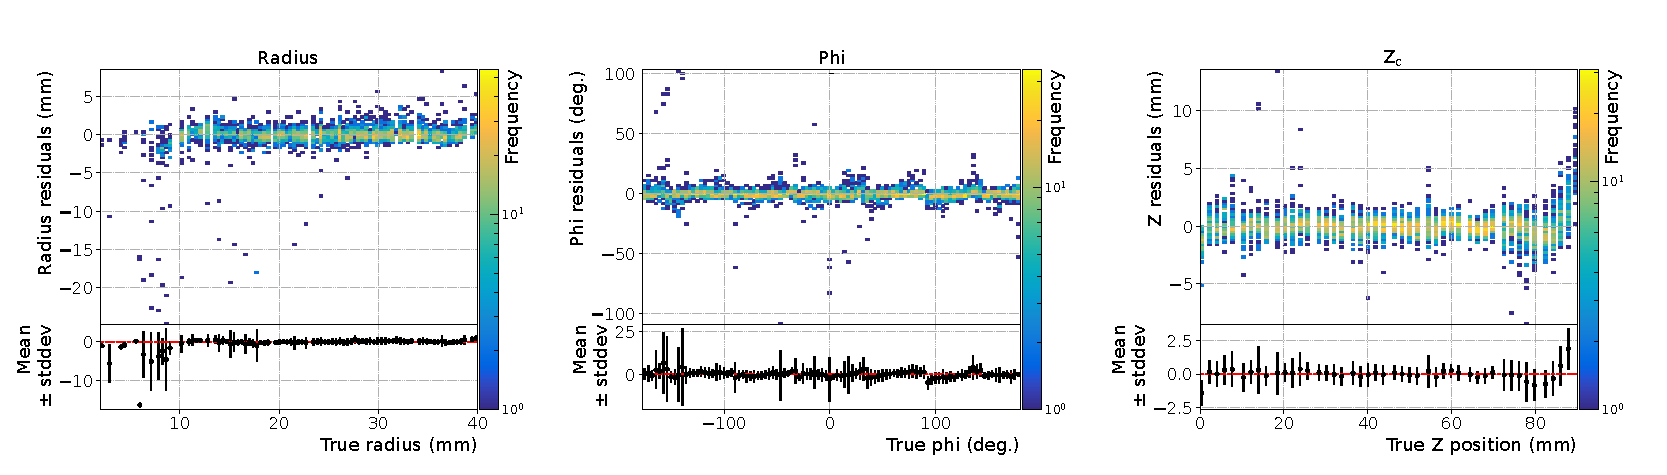
\includegraphics[width=\textwidth]{images/residuals_subplots_grouped.eps}
% \vspace*{2cm}% Give the correct figure height in cm
\caption{From left to right, residuals of the model predictions on the test-set for $r, \varphi$ and $\text{Z}_\text{c}$, respectively. The bottom plots show the mean value of the Y-projected bins along the X-axis, together with the standard deviation of the distribution.}
\label{fig:all_residuals}       % Give a unique label
\end{figure*}

\begin{table}
\centering
\caption{Train- and test-set RMSE metrics. Units are given in mm for radius and Z, unit-less for $\sin \varphi$ and $\cos \varphi$.}
\label{tab:rmse_metrics}       % Give a unique label
\begin{tabular}{lcc}
\hline\noalign{\smallskip}
\textbf{Target} & \textbf{\shortstack{Train set \\ RMSE}} & \textbf{\shortstack{Test set \\ RMSE}} \\
\noalign{\smallskip}\hline\noalign{\smallskip}
Radius (mm) & 1.2418 & 1.4828 \\
$\sin \varphi$ & 0.0828 & 0.0869 \\
$\cos \varphi$ & 0.0446 & 0.0550 \\
Z (mm) & 0.8147 & 1.1416 \\
\noalign{\smallskip}\hline
\end{tabular}
\end{table}
% \centering
% \caption{Test set metrics. Units are given  in mm for radius and Z, unitless for $\sin \varphi$ and $\cos \varphi$.}
% \label{tab:test_metrics}       % Give a unique label
% \begin{tabular}{lll}
% \hline\noalign{\smallskip}
% Target & RMSE & R²  \\
% \noalign{\smallskip}\hline\noalign{\smallskip}
% Radius & 1.4828 & 0.9679 \\
% $\sin \varphi$ & 0.0869 & 0.9846 \\
% $\cos \varphi$ & 0.0550 & 0.9941 \\
% Z & 1.1416 & 0.9980 \\
% \noalign{\smallskip}\hline
% \end{tabular}
% \end{table}

To understand how the reconstruction performs in the volume of A005, the 3D euclidean error for all points of the test-se is shown in \textbf{Fig.}~\ref{fig:3d_err_per_slice_seg}. The mean 3D euclidean error for the whole test set is $\operatorname{D}_\text{mean} = 1.88$ mm where $\operatorname{D}_\text{mean}$ is computed by switching back to euclidean coordinates.

\begin{figure}
\centering
\resizebox{0.30\textwidth}{!}{%
  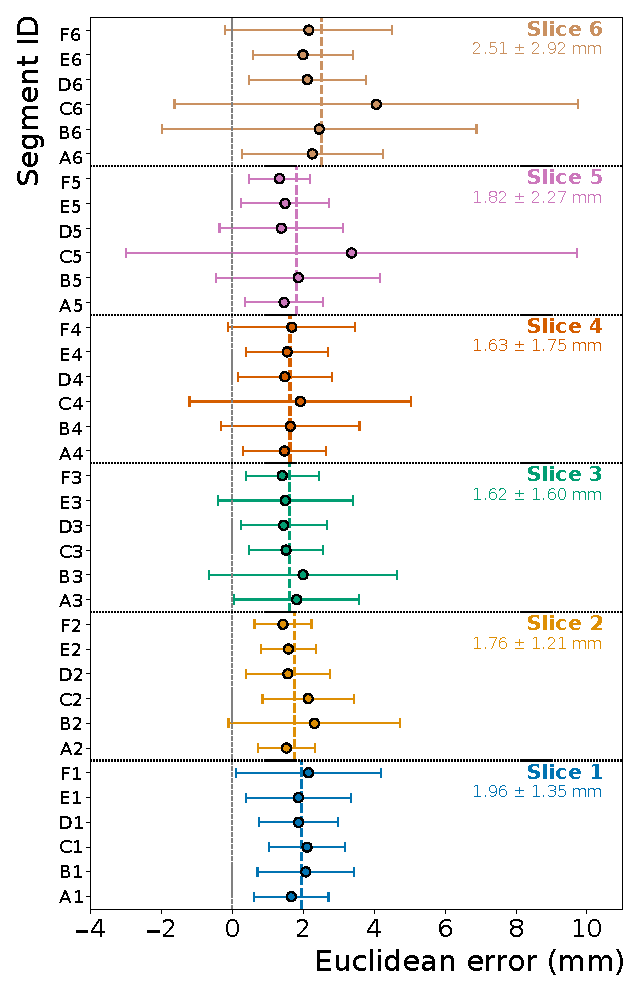
\includegraphics{images/slice_err_cblind.eps}
}
% If not, use
%\vspace{5cm}       % Give the correct figure height in cm
\caption{Euclidean error computed on test-set samples, for all segments of A005, gathered by slice. The colored dashed vertical lines represent the mean error of each slice, reported below the slice number. Error bars show the standard deviation of each bin's error distribution. Null euclidean error is represented by the gray vertical dashed line.}
\label{fig:3d_err_per_slice_seg}       % Give a unique label
\end{figure}

\section{Position reconstruction}
\label{sec:position_reconstruction}
Using collimated beams taken with A005 in horizontal orientation on the IPHC scanning table, it is possible to test the GBRT model on unseen data with more realistic conditions. Data were taken a few months before building A005 pulses database that was used to train the model. Thus, the gains of the segments could have shifted in the meantime. In addition to fold-1 events position reconstruction, fold-2 events position reconstruction will be presented. The pulses have a lower signal-to-noise ratio and this is a more challenging evaluation of the performance of the model.

Results will be presented by showing the reconstructed hit positions in different visualization planes, YX, YZ and XZ.

\subsubsection*{\underline{Collimated beam at $(\text{Z}_\text{c}, \text{X}_\text{c})= (10\pm0.02, -9\pm0.02)$ mm}}
\subsection{Fold-1 events}

Full-energy deposition fold-1 events are reconstructed by the trained GBRT model and the positions are shown in \textbf{Fig.}~\ref{fig:H_beam_10.0_-9.0_fold2_HitIndex1_and_fold1}. The effect of the segmentation lines are visible on YZ-plane \textbf{(a)} and YX-plane \textbf{(b)}. Fold-1 photoelectric effect does no occur on the segmentation lines, which explains this cut in the reconstructed interactions. 

% FOLD-1 3 SUBPLOTS FIGURE
% \begin{figure*}[htb]
% 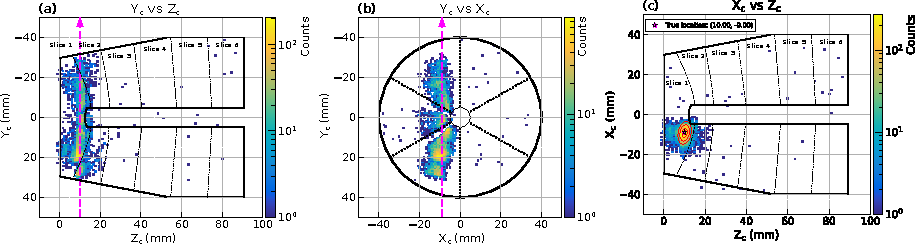
\includegraphics[width=\textwidth]{images/superimposed_D10,0_-9,0_fold1_3subplots_with_fit.pdf}
% % \vspace*{2cm}% Give the correct figure height in cm
%      \caption{\textbf{(a)} YZ-plane representation of the interactions along the collimated $\gamma$-ray beam. \textbf{(b)} YX-plane representation of the interactions along the collimated $\gamma$-ray beam. In \textbf{(a)} and \textbf{(b)}, the magenta arrows represent the position and direction of the collimated beam. \textbf{(c)} XZ-plane representation of the interactions along the collimated $\gamma$-ray beam. Magenta star represents the position of the beam, seen from above. Red contours from the 2D gaussian fit are shown. All color scales are logarithmic.}
% \label{fig:H_beam_10.0_-9.0}       % Give a unique label
% \end{figure*}

To evaluate the model's performance, a 2D gaussian fit is shown on \textbf{Fig.}~\ref{fig:H_beam_10.0_-9.0_fold2_HitIndex1_and_fold1}(c). Red contours of the fit are also shown.
%The fit results are presented in \textbf{Table}~\ref{tab:gaussian_fit_results_m1}.

% \begin{figure}
% \centering
% \resizebox{0.48\textwidth}{!}{%
%   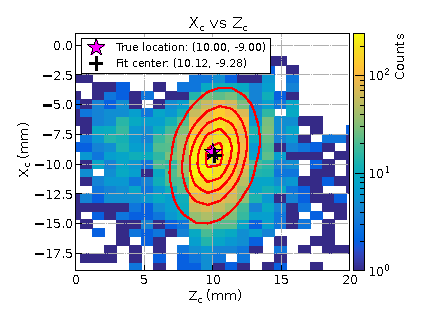
\includegraphics{images/h2d_ZX_zoom_and_fit_T-166,66_163,68_D10,0_-9,0_mlflow_Fold1.eps}
% }
% % If not, use
% %\vspace{5cm}       % Give the correct figure height in cm
% \caption{2D gaussian fit of the reconstructed positions of the photoelectric hits from a $^{137}$Cs collimated beam, in the XZ-plane. The true position of the beam in the detector's frame is shown as the magenta star. Gaussian fit center is shown as a black cross. Color scale is logarithmic.}
% \label{fig:XZ_horizontal_beam_2d_gaussian_fit}       % Give a unique label
% \end{figure}

\subsection{Fold-2 events}
For fold-2 events depositing the full incident $\gamma$-ray energy, the ordering of the interactions is uncertain as the incident gamma ray energy is over 255.5~keV. This is a result derived from the Compton kinematics. A probabilistic method is used to assign an interaction order based on the energy deposited by the two interactions:

\begin{enumerate}
    \item First hit is assigned to the highest energy deposit E\textsubscript{max} of the pair;
    \item Compton edge test is performed, meaning the maximum energy deposited (Compton edge energy E\textsubscript{ce}) is computed using \ensuremath{\text{E}_\text{tot} = \text{E}_1 + \text{E}_2} and a scattering angle $\theta = 180^\circ$. If E\textsubscript{max} $>$ E\textsubscript{ce}, order of interactions is inverted.
\end{enumerate}

This method results in approximately 60\% of correct fold-2 events ordering at 662 keV~\cite{Piqueras2004ADetectors}.
Pulses have a lower signal-to-noise ratio and this makes fold-2 events a robust evaluation of the performance of the GBRT model. \textbf{Fig.}~\ref{fig:H_beam_10.0_-9.0_fold2_HitIndex1_and_fold1} shows the reconstructed positions of the first interactions only from the fold-2 events, using the probabilistic ordering method described above. To limit the noise in the transient signals, data was filtered to keep fold-2 events with second hit not in the neighborhood of the first hit.

%\underline{Collimated beam at (Z\textsubscript{c},Y\textsubscript{c}) = (10, -9) mm}\\

% FOLD-2 3 SUBPLOTS FIGURE
% \begin{figure*}[htb]
% 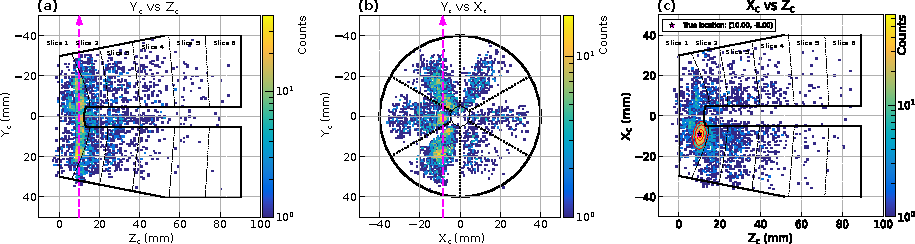
\includegraphics[width=\textwidth]{images/superimposed_D10,0_-9,0_fold2_HitIndex1_3subplots_with_fit.pdf}
% % \vspace*{2cm}% Give the correct figure height in cm
%      \caption{\textbf{(a)} YZ-plane representation of the interactions along the collimated $\gamma$-ray beam. \textbf{(b)} YX-plane representation of the interactions along the collimated $\gamma$-ray beam. In \textbf{(a)} and \textbf{(b)}, the magenta arrows represent the position and direction of the collimated beam. \textbf{(c)} XZ-plane representation of the collimated beam. Magenta star represents the position of the beam, seen from above. Red contours from the 2D gaussian fit are shown. All color scales are logarithmic.}
% \label{fig:H_beam_10.0_-9.0_fold2_HitIndex1}       % Give a unique label
% \end{figure*}

\begin{figure*}[htb]
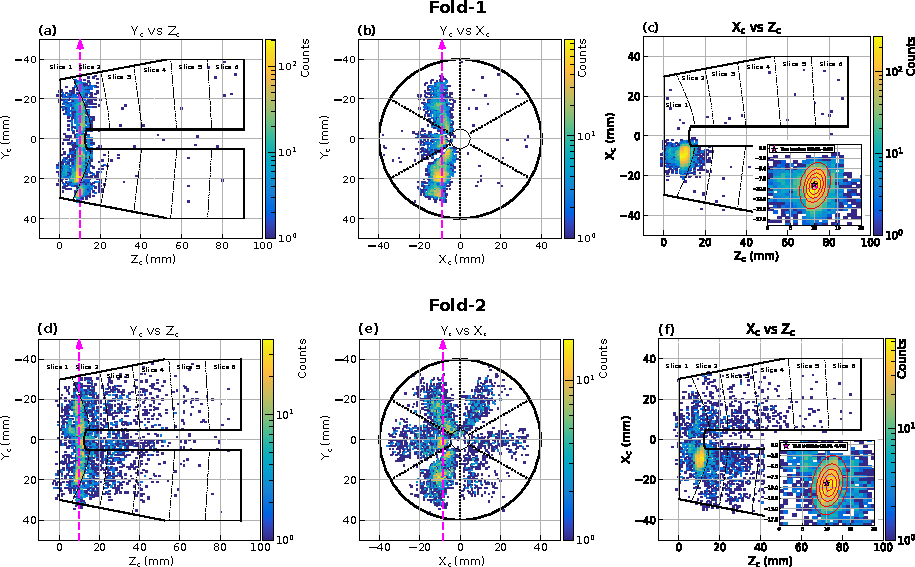
\includegraphics[width=\textwidth]{images/superimposed_D10,0_-9,0_fold2_HitIndex1_AND_fold1_3subplots_with_fit.pdf}
% \vspace*{2cm}% Give the correct figure height in cm
     \caption{\textbf{(a)} YZ-plane representation of the interactions along the collimated $\gamma$-ray beam. \textbf{(b)} YX-plane representation of the interactions along the collimated $\gamma$-ray beam. In \textbf{(a)} and \textbf{(b)}, the magenta arrows represent the position and direction of the collimated beam. \textbf{(c)} XZ-plane representation of the collimated beam. Magenta star represents the position of the beam, seen from above. Red contours from the 2D gaussian fit are shown inside inserts zooming on the beam spot, in \textbf{(c)} and \textbf{(f)}. \textbf{(a)}, \textbf{(b)} and \textbf{(c)} show the fold-1 reconstructed positions. \textbf{(d)}, \textbf{(e)} and \textbf{(f)} show the first-hit reconstructed position of fold-2 events. All color scales are logarithmic.}
\label{fig:H_beam_10.0_-9.0_fold2_HitIndex1_and_fold1}       % Give a unique label
\end{figure*}

% \begin{figure}
% \centering
% \resizebox{0.48\textwidth}{!}{%
%   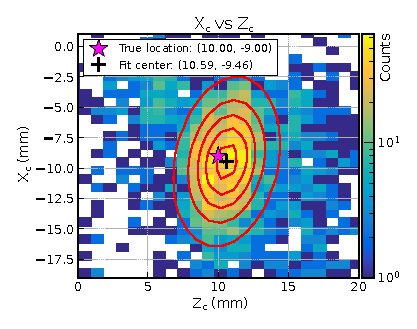
\includegraphics{images/h2d_ZX_zoom_and_fit_T-166,66_163,68_D10,0_-9,0_mlflow_Fold2_HitIndex1.eps}
% }
% % If not, use
% %\vspace{5cm}       % Give the correct figure height in cm
% \caption{2D gaussian fit of the reconstructed positions of the fold-2 events first hits from a $^{137}$Cs collimated beam, in the XZ-plane. The true position of the beam in the detector's frame is shown as the magenta star. Gaussian fit center is shown as a black cross. Color scale is logarithmic.}
% \label{fig:XZ_horizontal_beam_2d_gaussian_fit_Fold2_HitIndex1}       % Give a unique label
% \end{figure}

The results of the 2D gaussian fit for both fold-1 and fold-2 events reconstruction are given in \textbf{Table}~\ref{tab:gaussian_fit_results_combined}.

\begin{table}[ht]
\centering
\caption{2D Gaussian fit results for full-energy deposition fold-1 and fold-2 events reconstruction in the ZX-plane. The $\gamma$-ray beam is located at $(\text{Z}_\text{c}, \text{X}_\text{c}) = (10\pm0.02, -9\pm0.02)$. Fit values are given with their uncertainties in parenthesis notation. Theta corresponds to the rotation of the Gaussian.}
\label{tab:gaussian_fit_results_combined}
\begin{tabular}{lrr}
\hline\noalign{\smallskip}
\textbf{Parameter} & \textbf{Fold-1} & \textbf{Fold-2} \\
\noalign{\smallskip}\hline\noalign{\smallskip}
Amplitude & $262.644(937)$ & $49.330(300)$ \\
Mean X (mm) & $10.121(5)$ & $10.594(11)$ \\
Mean Y (mm) & $-9.278(10)$ & $-9.463(20)$ \\
Stddev X (mm) & $1.445(5)$ & $1.685(10)$ \\
Stddev Y (mm) & $2.707(10)$ & $3.276(20)$ \\
Theta (rad) & $-0.187(4)$ & $-0.150(6)$ \\
\noalign{\smallskip}\hline
\end{tabular}
\end{table}

\section{Conclusion}
Training an ensemble machine learning model on features extracted from pulses recorded on an AGATA detector, this work shows that a millimetric position reconstruction is possible by using features extracted from the pulses, without the use of grid-search or adaptative grid-search algorithms.

Models were combined and tested on the test-set, resulting in a 3D euclidean error of 1.88 mm. Their performance was also evaluated on a collimated beam of 662 keV $\gamma$ rays from a $^{137}$Cs source, both for fold-1 and 2 events with full-energy deposition, showing robustness of the method with features extracted from noisy pulses compared to what the model was trained with.

The parameter $\varphi$ was reconstructed from two independent models, the correctness of the identity \ensuremath{\sin^2 \varphi + \cos^2 \varphi = 1} was not enforced. While this is a limitation of current approach, this does not seem to prevent a correct hit azimuthal position reconstruction.
%
% For two-column wide figures use
% \begin{figure*}
% % Use the relevant command for your figure-insertion program
% % to insert the figure file. See example above.
% % If not, use
% % 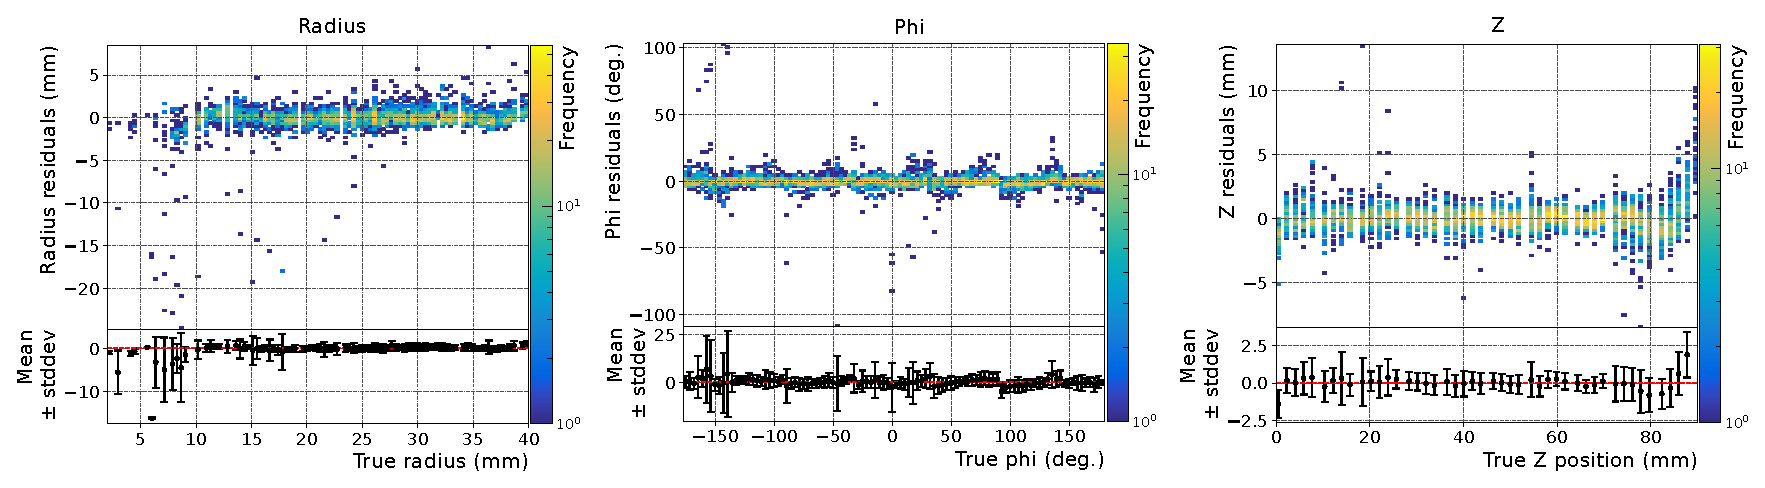
\includegraphics{images/residuals_grouped_title.eps}
% % \vspace*{5cm}       % Give the correct figure height in cm
% \caption{Please write your figure caption here}
% \label{fig:2}       % Give a unique label
% \end{figure*}
%
% For tables use
\section{Acknowledgements}
\label{sec:acknowledgements}
The authors are grateful for the important technical contributions of M.-H. Sigward, M. Filliger and F. Didierjean. The authors acknowledge support from Région Grand-Est and MIRION Technologies CANBERRA, Contracts N$^\circ$\,252911 and 260587, respectively.

%
% BibTeX users please use
\bibliographystyle{unsrt}
\bibliography{biblio}
% \printbibliography
\end{document}

% end of file template.tex

